\documentclass{article}

\usepackage[utf8]{inputenc}
\usepackage[T1]{fontenc}
\usepackage[spanish]{babel}
\usepackage{times}
\usepackage{wrapfig}
\usepackage{lmodern}
\usepackage{mathtools}
\usepackage{graphicx}
\usepackage[utf8]{inputenc}
\usepackage{color}
\usepackage{hyperref}
\usepackage{fancyhdr,lipsum}


\hypersetup{
    colorlinks=true, %set true if you want colored links
    linktoc=all,     %set to all if you want both sections and subsections linked
    linkcolor=blue,  %choose some color if you want links to stand out
}

\definecolor{gray97}{gray}{.97}
\definecolor{gray75}{gray}{.75}
\definecolor{gray45}{gray}{.45}

%definir los marcos, fondos, numero y demás de los códigos de SQL
\usepackage{listings} 
  \lstset{ frame=Ltb,
          framerule=0pt,
          aboveskip=0.5cm,
          framextopmargin=3pt,
          framexbottommargin=3pt,
          framexleftmargin=0.4cm,
          framesep=0pt,
          rulesep=.4pt,
          backgroundcolor=\color{gray97},
          rulesepcolor=\color{black},
          %
          stringstyle=\ttfamily,
          showstringspaces = false,
          basicstyle=\small\ttfamily,
          commentstyle=\color{gray45},
          keywordstyle=\bfseries,
          %
          numbers=left,
          numbersep=15pt,
          numberstyle=\tiny,
          numberfirstline = false,
          breaklines=true,
  }

% minimizar fragmentado de listados
\lstnewenvironment{listing}[1][]{\lstset{#1}\pagebreak[0]}{\pagebreak[0]}
\lstdefinestyle{consola}{basicstyle=\scriptsize\bf\ttfamily, backgroundcolor=\color{gray75}, }
\lstdefinestyle{C}{language=C,}

\title{Tarea 2.- Creación de la base de datos \textbf{URGENCIAS}}
\author{Antonio Muñoz Cubero}
 

\begin{document}
  \maketitle
    \pagenumbering{gobble}
      \pagestyle{fancy} 

\newpage
  \tableofcontents
    \lhead[BD URGENCIAS]{BD URGENCIAS}
    \lfoot[IES Francisco De Los Rios]{IES Francisco De Los Rios}
      \pagenumbering{arabic}

\newpage
  \section{Foto del Modelo Relacional}
    \begin{figure}[h]
      \centering
      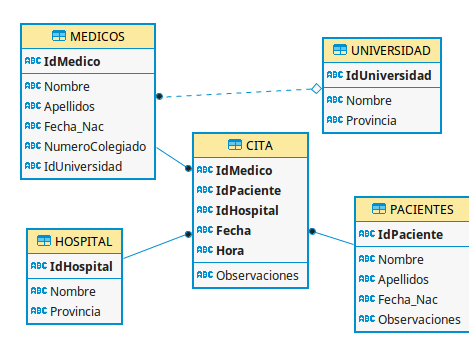
\includegraphics[scale = 1]{img/enunciado.png}
      \caption{Foto del Modelo Relacional desde el que partimos.}
    \end{figure}

\newpage
  \section{Creación de la Base de Datos}
    Entramos al cliente de MariaDB con el usuario que tengamos para trabjar, acto seguido empezaremos creando 
    la base de datos \textbf{urgencias} usando los siguientes comandos, después la seleccionamos y comenzamos la creación de las tablas. 
    \begin{listing}[style=consola, numbers=none]
    MariaDB [(none)]> CREATE DATABASE IF NOT EXISTS urgencias;

    MariaDB [(none)]> USE urgencias;

    \end{listing}

  \section{Creación de las tablas}
    En este caso, las tablas debemos de comenzar a crearlas teniendo en cuenta si hay claves que dependan de otras o no, en nuestro caso, empezaremos creando 
    la taba \textbf{Universidad}, que no depende de ninguna y posteriormente la tabla \textbf{Medico}, que depende de \textbf{Universidad}.
    \subsection{Tabla 'Universidad'}
      \begin{lstlisting}[style=C]
        CREATE TABLE IF NOT EXISTS Universidad(
          idUniversidad INT(10) NOT NULL AUTO_INCREMENT,
          nombre VARCHAR(100) NOT NULL,
          provincia VARCHAR(100) NOT NULL,
          CONSTRAINT pk_Universidad_idUniversidad PRIMARY KEY (idUniversidad),
          CONSTRAINT u_Universidad_nombre UNIQUE (nombre)
        )
        ENGINE = InnoDB
        COMMENT ='Tabla donde se definen las universidades que hay en la base de datos'
        ;
      \end{lstlisting}

  \newpage
    \subsection{Tabla 'Medico'}
      \begin{lstlisting}[style=C]
        CREATE TABLE IF NOT EXISTS Medico(
          idMedico INT (10) NOT NULL AUTO_INCREMENT,
          nombre VARCHAR(100) NOT NULL,
          apellidos VARCHAR(100) NOT NULL,
          fechaNacimiento DATE NOT NULL,
          numeroColegiado INT(15) NOT NULL,
          idUniversidad INT(10) NOT NULL,
          CONSTRAINT pk_Medico_idMedico PRIMARY KEY (idMedico),
          CONSTRAINT fk_Medico_idUniversidad FOREIGN KEY (idUniversidad) REFERENCES Universidad (idUniversidad),
          CONSTRAINT u_Medico_numeroColegiado UNIQUE (numeroColegiado)
        )
        ENGINE = InnoDB
        COMMENT ='Tabla donde almacenamos los datos de los medicos en la base de datos'
        ;
      \end{lstlisting}

  %\newpage
    \subsection{Tabla 'Hospital'}
      \begin{lstlisting}[style=C]
        CREATE TABLE IF NOT EXISTS Hospital(
          idHospital INT (10) NOT NULL,
          nombre VARCHAR(100) NOT NULL,
          provincia VARCHAR(100) NOT NULL,
          CONSTRAINT pk_Hospital_idHospital PRIMARY KEY (idHospital)
        )
        ENGINE = InnoDB
        COMMENT = 'Tabla donde almacenamos los hospitales que hay en la base de datos'
        ;
      \end{lstlisting}

  \newpage
    \subsection{Tabla 'Paciente'}
      \begin{lstlisting}[style=C]
        CREATE TABLE IF NOT EXISTS Paciente(
          idPaciente INT(10) NOT NULL,
          nombre VARCHAR(100) NOT NULL,
          apellidos VARCHAR(100) NOT NULL,
          fechaNacimiento DATE NOT NULL,
          observaciones TEXT DEFAULT 'Ninguna',
          CONSTRAINT pk_Paciente_idPaciente PRIMARY KEY (idPaciente)
        )
        ENGINE = InnoDB
        COMMENT = 'Tabla donde almacenamos los pacientes que hay en la base de datos'
        ;
      \end{lstlisting}

    \subsection{Tabla 'Cita'}
      \begin{lstlisting}[style=C]
        CREATE TABLE IF NOT EXISTS Cita(
          idMedico INT(10) NOT NULL,
          idPaciente INT(10) NOT NULL,
          idHospital INT(10) NOT NULL,
          fecha DATE NOT NULL,
          hora TIME NOT NULL,
          observaciones TEXT DEFAULT 'Ninguna',
          CONSTRAINT pk_Cita_idMedico_idPaciente_idHospital PRIMARY KEY (idMedico, idPaciente, idHospital),
          CONSTRAINT fk_Cita_idMedico FOREIGN KEY (idMedico) REFERENCES Medico (idMedico),
          CONSTRAINT fk_Cita_Paciente FOREIGN KEY (idPaciente) REFERENCES Paciente (idPaciente),
          CONSTRAINT fk_Cita_idHospital FOREIGN KEY (idHospital) REFERENCES Hospital (idHospital)
        )
        ENGINE = InnoDB
        COMMENT = 'Tabla donde almacenamos las citas que hay en la base de datos, su clave es la union la varias pk de otras tablas'
        ;
      \end{lstlisting}
  \newpage
    \section{Insercción de Datos}
      En el apartado de Insercción, opté por la opción de crear archivos \textbf{CSV}, ya que me parece mucho más práctico a la hora de 
      insertar datos de primera hora, los archivos están adjuntos en la entrega y son importados usando los siguientes comandos SQL:
      \\
      \\
      \textbf{Hay dos rutas, ya que importé los archivos tanto en Linux como en Windows. Solo ha de usarse una de las dos, dependiendo 
      del sistema operativo en el que se encuentre.}
      \\
      \\
      \textit{De esta manera habría que añadir el id manualmente en el archivo.}
      \begin{lstlisting}[style=C]
        LOAD DATA LOCAL INFILE '/home/...'
        LOAD DATA LOCAL INFILE 'C:/..'
        INTO TABLE urgencias.Universidad
        FIELDS TERMINATED BY ','
        LINES TERMINATED BY '\n'
        (@ignorado, nombre, provincia)
        IGNORE 1 ROWS
        ;
      \end{lstlisting}
      \textit{De esta manera habría que añadir el id manualmente en el archivo.}
      \begin{lstlisting}[style=C]
        LOAD DATA LOCAL INFILE '/home/...'
        LOAD DATA LOCAL INFILE 'C:/..'
        INTO TABLE urgencias.Universidad
        FIELDS TERMINATED BY ','
        LINES TERMINATED BY '\n'
        (@ignorado, nombre, provincia)
        ;
      \end{lstlisting}
      \textit{Si por ejemplo, en la tabla \textbf{Medico}, insertaramos mal un campo, por ejemplo, su \textbf{fecha de nacimiento}, para actualizarlo, se 
      haría tal que así:}
      \begin{lstlisting}[style=C]
        UPDATE urgencias.Medico
        SET fechaNacimiento='1999-05-2' WHERE idMedico = 1
        ;
      \end{lstlisting}
  \newpage
    \section{Modelo E-R desde Dbeaver}
      \begin{figure}[h]
        \centering
        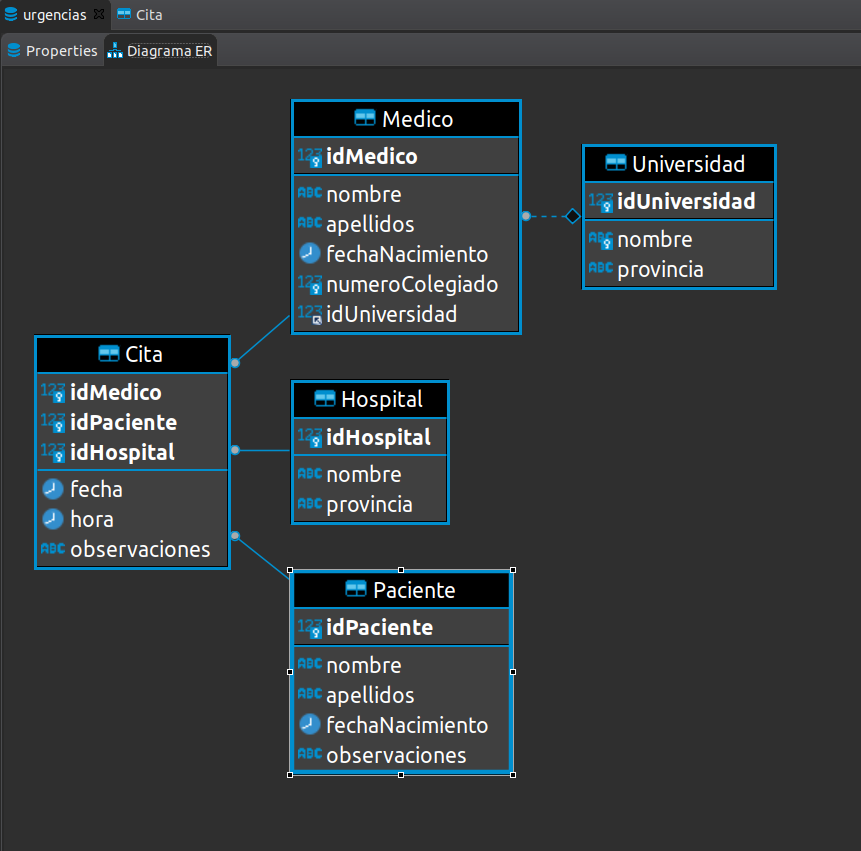
\includegraphics[scale = 0.75]{img/modelo-E-R.png}
        \caption{Modelo E-R desde Dbeaver}
      \end{figure}
  \newpage
    \section{Vista de los registros introducidos}
      \begin{figure}[h]
        \centering
        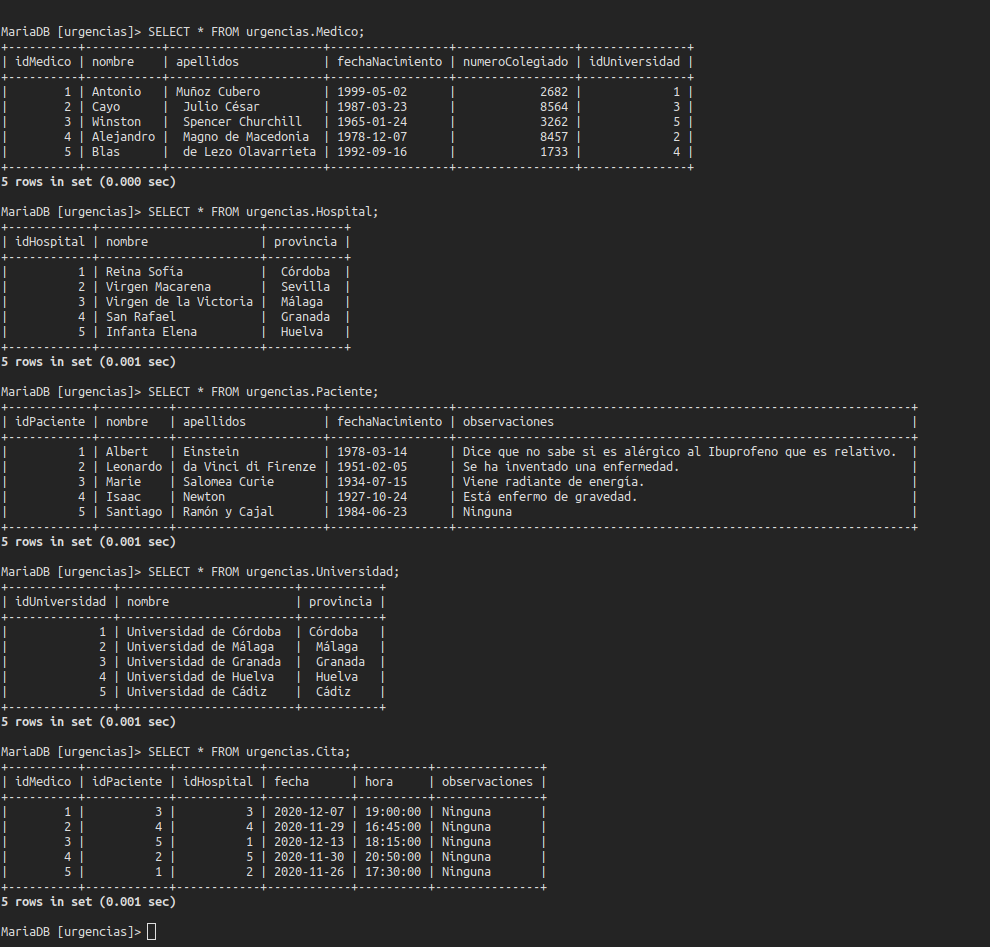
\includegraphics[scale = 0.7]{img/select.png}
        \caption{Consulta SELECT de todas las tablas.}
      \end{figure}

  \newpage
    \listoffigures

\end{document}